\begin{figure}[H]
  \centering

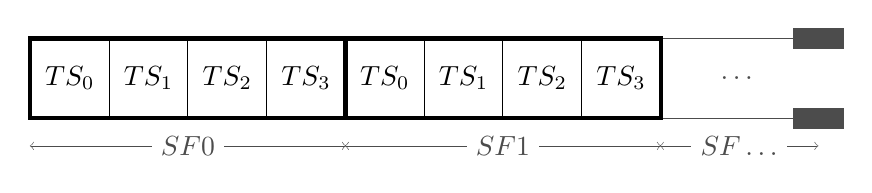
\begin{tikzpicture}[
  timeslot/.style={draw, rectangle, minimum size=1cm},
  arr/.style={help lines,black!70,<->},
]

\foreach [evaluate={\ts=int(mod(\i, 4))}] \i in {0,...,7} {
  \node (ts\i) [timeslot] at (\i, 0) {$TS_{\ts}$};
}
\node (ts8) [minimum height=1cm, minimum width=2cm, black!70] at (8.5, 0) {\ldots};
\draw[help lines, black!70]
  (ts8.north west) -- (ts8.north east) node[fill=white, black!70] {$\ldots$};
\draw[help lines, black!70]
  (ts8.south west) -- (ts8.south east) node[fill=white, black!70] {$\ldots$};

\draw[ultra thick] 
  (ts0.south west) rectangle (ts3.north east)
  (ts4.south west) rectangle (ts7.north east);

\draw[arr]
  ([yshift=-10pt]ts0.south west) -- node[fill=white] {$SF0$} ([yshift=-10pt]{ts3.south east});
\draw[arr]
  ([yshift=-10pt]ts4.south west) -- node[fill=white] {$SF1$} ([yshift=-10pt]{ts7.south east});
\draw[arr]
  ([yshift=-10pt]ts8.south west) -- node[fill=white] {$SF\ldots$} ([yshift=-10pt]{ts8.south east});

\end{tikzpicture}

\caption{Slotframes representation\label{fig:timeslots}}
\end{figure}
